\subsection{Sensor}
I dette afsnit diskuteres forskellige valg af sensorer, deres specifikationer og der dannes grundlag for valg af sensor. \newline

\subsubsection{Kriterier for valg af sensor:} 
\begin{enumerate}
	\item[•]Digital eller analog		
	\item[•]Præcision på sensoren 
	\item[•]Måleafstand			
	\item[•]Driftsspænding
	\item[•]Pris
\end{enumerate} 

I forbindelse med kriterierne sat for valg af sensor samt kravene i kravspecifikationen er temperatur sensor DALLAS18b20 (DS18b20) valgt til måling af vandrør. Alle sensorer i tabel 3.1 er digitale hvoraf dem, kun DS18b20 kan monteres ved hjælp af Tht (Through hole technology). Dette kan være en fordel under montering. De digitale sensorer vist i nedenstående tabel er valgt fordi de er nemmere at forbinde i forhold til analoge sensorer som kan påvirkes af kredsløbet.

 
\begin{table}[h]
\centering
\begin{tabular}{|l|l|l|l|l|}
\hline
 & LM9523 & LM53DIMA & LM86CIM & Ds18b20 \\ \hline
Digital & Ja & Ja & Ja & Ja \\ \hline
Præcision & $\pm$1 $^{\circ}$C, $\pm$2.5 $^{\circ}$C & $\pm$1 $^{\circ}$C, $\pm$3 $^{\circ}$C & $\pm$1 $^{\circ}$C, $\pm$3 $^{\circ}$C & \begin{tabular}[c]{@{}l@{}}$\pm$0,5$^{\circ}$C (ved -10 \\ til +85$^{\circ}$C)\end{tabular} \\ \hline
Driftstemperatur & 0 $^{\circ}$C til +85 $^{\circ}$C & 0 $^{\circ}$C til 85 $^{\circ}$C & 0 $^{\circ}$C til 85 $^{\circ}$C & -55$^{\circ}$C til 125$^{\circ}$C \\ \hline
Montering & SMD & SMD & SMD & Tht \\ \hline
Pris & 18,10 DKK & 18,85 DKK & 11,864 DKK & 35,20 DKK \\ \hline
Driftsspænding & 3,0 V til 3,6 V & 3,0 V til 3,6 V & 3,0 V til 3,6 V & 3,0 V til 5,5V \\ \hline
\end{tabular}
\caption{Tabel over mulige valg af sensorer}
\label{sensor_tabel}
\end{table}
\newpage
  

DS18b20 i kontrast til de resterende vist i tabel 3.1 besidder den mest nøjagtige præcision samt opfylder kravene i kravspecifikationen med en måleafstand på 0-25$^{\circ}$ C. \newline
Ds18b20 er en digital temperatur sensor som sender målinger over 9-12 bit og anbefales en spænding mellem 3,0-5,5 V. \newline
Sensoren har en driftstemperatur mellem -55-125$^{\circ}$ og har en præcisions temperatur på $\pm$0,5$^{\circ}$C ved -10 til +85$^{\circ}$. Sensoren kommunikere via en 1-Wire bus forbindelse som kun kræver en enkelt data forbindelse for at kommunikere med mikroprocessoren. Denne ene data forbinelse kan samtidig anvendes som strømforsyning til sensoren. Dette forstås som "parasite power". Dette muliggør også for ikke at anvende ekstern strømforsyning. 
Denne ene forbindelse gør den ideél netop i videreudviklingen af produktet hvis flere sensorer skal forbindes til samme ledning.

\begin{figure}[h!]
  \centering
  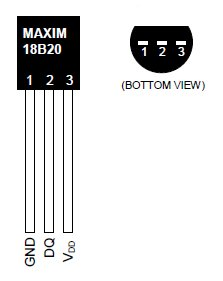
\includegraphics[width=0.3\textwidth]{figures/ds18b20-pinout.jpg}
  \caption{Tegning over DS18b20 temperatur sensor.}
  \label{ds18b20_pins}
\end{figure} 

Til målingen af rum temperaturen er DHT11 valgt. Det er en digital sensor som måler både temperatur samt ændringer i luftfugtigheden. Denne sensor kræver en strømtilførsel på 3-5 V. \newline
Den kan måle temperaturændringer inden for 0-50$^{\circ}$ med en præcision på $\pm$2$^{\circ}$C, samt måle luftfugtighedsændringer inden for 20-80\% fugtighed med en præcision på 5\%. 

\begin{figure}[h!]
  \centering
  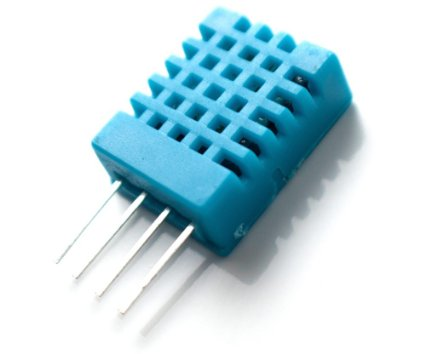
\includegraphics[width=0.3\textwidth]{figures/DHT11.jpg}
  \caption{DHT11 temperatur og luftfugtigheds sensor.}
  \label{dht11_billede}
\end{figure} 
   






\newpage
